\section{Problem 4: A Simple Portfolio Choice Problem}
\begin{enumerate}
\item 
Yes, since the CRRA utility function is convex and the set of possible $\alpha$ is a closed convex set. The problem is convex means that if a local minimum is found, it would be the global minimum as well.

\item
\begin{enumerate}
\item 
Note that $w_0$ is not random, we can pull it out of the expectation operator. The problem becomes
\begin{equation*}
	\max_\alpha\left\{w_0^\phi\mathbb E\left[\frac{1}{\phi}[1+r^f+\alpha(r-r^f)]^\phi\right]\right\}.
\end{equation*}
Notice that $w_0$ is just a constant independent of $\alpha$, the optimal portfolio share is independent of initial wealth.

\item
The optimal portfolio share is $\alpha^*=2.7331>1$, i.e. the agent short-sells the risk-free asset (i.e. borrow) and buy the risky portfolio. 
\begin{center}
\begin{figure}[htbp]
\begin{center}
	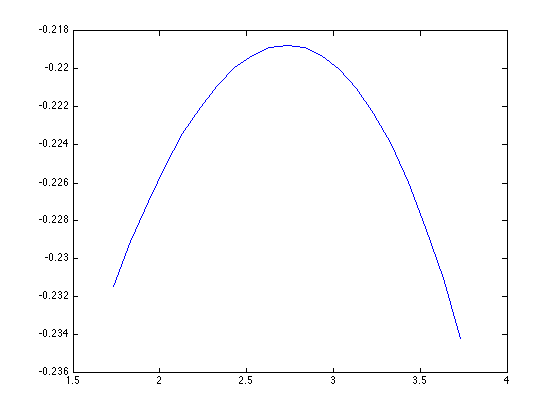
\includegraphics[width=10cm]{Figure/Q4_2b.png}
\end{center}
\end{figure}
\end{center}
\end{enumerate}

\item
\begin{enumerate}
\item
The constraint implies the agent cannot borrow or short sell.

\item
The solutions solved by \texttt{fminbnd} and \texttt{fmincon} are respectively 0.9999 and 1. The solutions are different because the constraint in \texttt{fminbnd} is $0<\alpha<1$ while in \texttt{fmincon} it is $0\le\alpha\le1$.

\item
Since the agent chooses to borrow when the constraint is not imposed, the constraint is binding. The best the agent can do is to invest as much as one can in the risky asset, thus yielding $\alpha^*=1$.

\end{enumerate}

\end{enumerate}
